\documentclass[aspectratio=169]{beamer}

\usepackage[utf8]{inputenc}

\usepackage{fontawesome5}
\usepackage{verbatim}
\usepackage{siunitx}
\usepackage{tikz, tikz-3dplot, tikz-uml}
\usepackage{pgffor}

\usetikzlibrary{calc, intersections, shapes, positioning}

%Information to be included in the title page:
\title{Layered Depth Images als Ad hoc Rendering für Punktwolken}
\author{Mario Henze}
\institute{Professur für Computergrafik und Visualisierung}
\date{2020}



\begin{document}

\frame{\titlepage}

\begin{frame}
    \frametitle{Gliederung}
    \begin{enumerate}
        \item Untersuchung klassischer Punktrender Verfahren
        \item Einführung Image based Rendering
        \item Motivation des hybriden Ansatzes
        \item Vorstellung des Viewmorphing nach McMillan
        \item Konzeption
        \item Auswertung
        \item Demo
    \end{enumerate}
\end{frame}

\begin{frame}
    \frametitle{QSplat}
    \begin{itemize}
        \item von Rusinkiewicz und Levoy entwickeltes Verfahren für Punktwolkenrendering
        \item effizientes Zeichnen durch Hierarchie von Begrenzungskugeln
        \item Vorverarbeitung notwendig
        \item Oberflächennormalen werden aus generiertem Dreiecksnetz gewonnen
        \item Ermöglicht Verdeckung von Lochartefakten
    \end{itemize}
\end{frame}

\begin{frame}
    \frametitle{Goswami}
    \begin{itemize}
        \item von Goswami et al.\ entwickeltes Punktwolkenrendering
        \item lokale Zusammenfassung von Punkten
        \item KD-Baum als Hierarchie von Punktclustern
        \item Quantisierung entlang der Koordinatenachsen ermöglicht parallele Bearbeitung
        \item Rendering erreicht variablen Detailgrad durch Prioritätswarteschlange
        \item Expansion der Baumknoten bis ausreichende Punktdichte erreicht
    \end{itemize}
\end{frame}

\begin{frame}
    \frametitle{Discher \& GBuffer}
    \begin{itemize}
        \item Punktwolkenrendering mit Fokus auf VR von Discher et al.\ entwickelt
        \item Renderprozess läuft in drei Phasen ab
        \item Auswahl einer repräsentativen Untermenge \& Culling
        \item Erstellen von G-Buffers als Zwischenrepräsentation
        \item Nachbearbeitung und finales Zeichnen
    \end{itemize}
\end{frame}

\begin{frame}
    \frametitle{Wimmer Instant Points}
    \begin{itemize}
        \item Wimmer und Scheiblauer Verfahren ohne Vorverarbeitung
        \item möglichst große Menge an Punkten mit interaktiven Bildraten
        \item Memory Optimized
        Sequential Point Trees (MOSPT) und verschachtelte Octrees als Datenstrukturen
        \item lokale Zusammenfassung durch Fehlermetrik
        \item Kombination von MOSPT und Octrees um statische Annahmen der MOSPT abzumildern
    \end{itemize}
\end{frame}

\begin{frame}
    \frametitle{Image based Rendering Review}
    \begin{itemize}
        \item Review von Heung-Yeung und Sing Bing
        \item stellt Spektrum der Image based Rendering Ansätze dar
        \item Einführung der plenoptischen Funktion
        \item Einordnung anhand der Parameteranzahl
    \end{itemize}
    \includegraphics[width=\linewidth]{images/review_spectrum}
\end{frame}

\begin{frame}
    \frametitle{McMillanWarping}
    \begin{itemize}
        \item von McMillan in verschiedenen Arbeiten entwickelte Datenstruktur
        \item sog. Layered Depth Images
        \item ermöglicht Zusammenfassung von Bildern mit verschiedenen Perspektiven
        \item erlaubt Bildsynthese für neue Ansichten
        \item Verdeckungsartefakte und Lochbildung vorhanden
    \end{itemize}
\end{frame}

\begin{frame}
    \frametitle{LDI Datenstruktur}
    \begin{itemize}
        \item Chun-Fa et al.\ Viewmorphing Verfahren
        \item Referenzbilder aus verschiedenen Perspektiven tasten Tiefenprofil unterschiedlich dicht ab
        \item Einordnung in einen LDI Baum
        \item Auswahl von Referenzbildern mit ähnlicher Tiefenauflösung zum Zielausschnitt
    \end{itemize}
\end{frame}

\begin{frame}
    \frametitle{Motivation}
    \begin{itemize}
        \item Punktwolkenrendering Methode für grundlegende Bildsynthese notwendig
        \item Image based Rendering für VR besonders lohnenswert
        \item Entwicklung eines hybriden Ansatzes
        \item Neuinterpretation des LDI als blickabhängige Punktwolke im Bildraum
        \item Viewmorphing kann somit auf Punktwolke übertragen werden
        \item Wiederverwendung des CGV Punktwolkenrenderer
    \end{itemize}
\end{frame}

\begin{frame}
    \frametitle{Plenoptic Modelling}

    \begin{columns}
    \column{.5\linewidth}
        \begin{equation}
            P_7 = P(V_x, V_y, V_z, \theta, \Phi, \lambda, t)
        \end{equation}
        
        \vspace{.5cm}

        \begin{description}[style=sameline]
            \item[\( V_x, V_y, V_z \)] mögliche Position der Kamera
            \item[\( \theta, \Phi \)] Winkel eines Sichtstrahls
            \item[\( \lambda \)] Wellenlänge des Lichts
            \item[\( t \)] Zeitpunkt der Beobachtung
        \end{description}
    \column{.5\linewidth}
        \begin{itemize}
            \item Beschreibung der Szene unabhängig vom Betrachter
            \item Sampling durch plenoptische Funktion
            \item herkömmliches Bild ist unvollständige und diskrete Abtastung dieser Funktion
            \item Image based Rendering nach McMillan versucht plenoptische Funktion zu rekonstruieren
        \end{itemize}
    \end{columns}
\end{frame}

\begin{frame}
    \frametitle{Plenoptic Modelling}
    \centering
    \includegraphics[width=.9\linewidth]{images/LytroVolumeTracer_VolumeSam}
\end{frame}

\begin{frame}
    \frametitle{Lochkamera}
    \begin{figure}
        \centering
        \tdplotsetmaincoords{70}{110}
        \resizebox{.8\linewidth}{!}{\begin{tikzpicture}[
        tdplot_main_coords,
        poi/.style = {circle, inner sep=1.5pt}
    ]
    %\draw[->] (0, 0, 0) -- (8, 0, 0) node[anchor = north]{x};
    %\draw[->] (0, 0, 0) -- (0, 8, 0) node[anchor = west]{y};
    %\draw[->] (0, 0, 0) -- (0, 0, 8) node[anchor = south]{z};
    \node[poi, fill=gray, label=below:{Brennpunkt}] (focal) at (0, 0, 0) {};
    % image corners
    \node[poi, fill=red] (ul) at (-4, 10, 2.25) {};
    \node[poi, fill=blue] (ur) at (4, 10, 2.25) {};
    \node[poi, fill=green] (lr) at (4, 10, -2.25) {};
    \node[poi, fill=yellow] (ll) at (-4, 10, -2.25) {};
    % sensor corners
    \node[poi, fill=red] (sul) at (-2, 5, 1.125) {};
    \node[poi, fill=blue] (sur) at (2, 5, 1.125) {};
    \node[poi, fill=green] (slr) at (2, 5, -1.125) {};
    \node[poi, fill=yellow] (sll) at (-2, 5, -1.125) {};
    % projection corners
    \node[poi, fill=green] (pul) at (-2, -5, 1.125) {};
    \node[poi, fill=yellow] (pur) at (2, -5, 1.125) {};
    \node[poi, fill=red] (plr) at (2, -5, -1.125) {};
    \node[poi, fill=blue] (pll) at (-2, -5, -1.125) {};
    % coords of image
    %\draw[->] (focal) -- (ul);
    %\draw[->] (ul) -- ++(2,0,0);
    %\draw[->] (ul) -- ++(0,0,-2);
    % image borders
    \draw (ul) -- (ur);
    \draw (ll) -- (lr);
    \draw (ul) -- (ll);
    \draw (ur) -- (lr);
    % view frustum
    \draw (focal) -- (sul);
    \draw (focal) -- (sur);
    \draw (focal) -- (slr);
    \draw (focal) -- (sll);
    \draw (sul) -- (ul);
    \draw (sur) -- (ur);
    \draw (slr) -- (lr);
    \draw (sll) -- (ll);
    % sensor edges
    \draw (sul) -- (sur);
    \draw (sll) -- (slr);
    \draw (sul) -- (sll);
    \draw (sur) -- (slr);
    % projection edges
    \draw[dotted] (pul) -- (pur);
    \draw[dotted] (pll) -- (plr);
    \draw[dotted] (pul) -- (pll);
    \draw[dotted] (pur) -- (plr);
    % view frustum
    \draw[dotted] (focal) -- (pul);
    \draw[dotted] (focal) -- (pur);
    \draw[dotted] (focal) -- (plr);
    \draw[dotted] (focal) -- (pll);
\end{tikzpicture}}%
        \label{fig:pinholecamera}
    \end{figure}
\end{frame}

\begin{frame}
    \frametitle{Layered Depth Image}
    \begin{columns}
    \column{.7\linewidth}
        \begin{figure}
            \centering
            \tdplotsetmaincoords{70}{110}
            \resizebox{\linewidth}{!}{\begin{tikzpicture}[
        tdplot_main_coords,
        poi/.style = {draw, shape = circle}
    ]
    %\draw[->] (0, 0, 0) -- (8, 0, 0) node[anchor = north]{x};
    %\draw[->] (0, 0, 0) -- (0, 8, 0) node[anchor = west]{y};
    %\draw[->] (0, 0, 0) -- (0, 0, 8) node[anchor = south]{z};
    \node (focal) at (0, 0, 0) {};
    % image corners
    \node (ul) at (-4, 10, 2.25) {};
    \node (ur) at (4, 10, 2.25) {};
    \node (lr) at (4, 10, -2.25) {};
    \node (ll) at (-4, 10, -2.25) {};
    % sensor corners
    \node (sul) at (-2, 5, 1.125) {};
    \node (sur) at (2, 5, 1.125) {};
    \node (slr) at (2, 5, -1.125) {};
    \node (sll) at (-2, 5, -1.125) {};
    % coords of image
    %\draw[->] (focal) -- (ul);
    %\draw[->] (ul) -- ++(2,0,0);
    %\draw[->] (ul) -- ++(0,0,-2);
    % image borders
    \draw[dotted] (ul.center) -- (ur.center);
    \draw[dotted] (ll.center) -- (lr.center);
    \draw[dotted] (ul.center) -- (ll.center);
    \draw[dotted] (ur.center) -- (lr.center);
    % view frustum
    \draw[dotted] (focal.center) -- (sul.center);
    \draw[dotted] (focal.center) -- (sur.center);
    \draw[dotted] (focal.center) -- (slr.center);
    \draw[dotted] (focal.center) -- (sll.center);
    \draw[dotted] (sul.center) -- (ul.center);
    \draw[dotted] (sur.center) -- (ur.center);
    \draw[dotted] (slr.center) -- (lr.center);
    \draw[dotted] (sll.center) -- (ll.center);
    % sensor edges
    \draw[] (sul.center) -- (sur.center);
    \draw[] (sll.center) -- (slr.center);
    \draw[] (sul.center) -- (sll.center);
    \draw[] (sur.center) -- (slr.center);
    % sensor grid
    %\draw[dotted] ($ (sul)!.25!(sll) $) -- ($ (sur)!.25!(slr) $);
    \foreach \n in {1,...,8}{
        \draw[] ($ (sul)!.125*\n!(sll) $) -- ($ (sur)!.125*\n!(slr) $);};
    \foreach \n in {1,...,16}{
        \draw[] ($ (sul)!.0625*\n!(sur) $) -- ($ (sll)!.0625*\n!(slr) $);};
    % world grid
    %\draw[dotted] ($ (sul)!.25!(sll) $) -- ($ (sur)!.25!(slr) $);
    \foreach \n in {1,...,8}{
        \draw[dotted] ($ (ul)!.125*\n!(ll) $) -- ($ (ur)!.125*\n!(lr) $);};
    \foreach \n in {1,...,16}{
        \draw[dotted] ($ (ul)!.0625*\n!(ur) $) -- ($ (ll)!.0625*\n!(lr) $);};
    % first example ray --> "f" as prefix
    % highlight sensor cell
    % calculate points on border
    \node (fslb1) at ($ (sul)!.125*1!(sll) $) {};
    \node (fslb2) at ($ (sul)!.125*2!(sll) $) {};
    \node (fsrb1) at ($ (sur)!.125*1!(slr) $) {};
    \node (fsrb2) at ($ (sur)!.125*2!(slr) $) {};

    \node (fsul) at ($ (fslb1)!.0625*1!(fsrb1) $) {};
    \node (fsll) at ($ (fslb2)!.0625*1!(fsrb2) $) {};
    \node (fslr) at ($ (fslb2)!.0625*2!(fsrb2) $) {};
    \node (fsur) at ($ (fslb1)!.0625*2!(fsrb1) $) {};
    \filldraw[draw=red, fill=red!20] (fsul.center) -- (fsll.center) -- (fslr.center) -- (fsur.center) -- cycle;
    % highlight world cell
    % calculate points on border
    \node (flb1) at ($ (ul)!.125*1!(ll) $) {};
    \node (flb2) at ($ (ul)!.125*2!(ll) $) {};
    \node (frb1) at ($ (ur)!.125*1!(lr) $) {};
    \node (frb2) at ($ (ur)!.125*2!(lr) $) {};

    \node (ful) at ($ (flb1)!.0625*1!(frb1) $) {};
    \node (fll) at ($ (flb2)!.0625*1!(frb2) $) {};
    \node (flr) at ($ (flb2)!.0625*2!(frb2) $) {};
    \node (fur) at ($ (flb1)!.0625*2!(frb1) $) {};
    \filldraw[draw=red, fill=red!20] (ful.center) -- (fll.center) -- (flr.center) -- (fur.center) -- cycle;

    % another example ray --> "a" as prefix
    % highlight sensor cell
    % calculate points on border
    \node (aslb1) at ($ (sul)!.125*5!(sll) $) {};
    \node (aslb2) at ($ (sul)!.125*6!(sll) $) {};
    \node (asrb1) at ($ (sur)!.125*5!(slr) $) {};
    \node (asrb2) at ($ (sur)!.125*6!(slr) $) {};

    \node (asul) at ($ (aslb1)!.0625*11!(asrb1) $) {};
    \node (asll) at ($ (aslb2)!.0625*11!(asrb2) $) {};
    \node (aslr) at ($ (aslb2)!.0625*12!(asrb2) $) {};
    \node (asur) at ($ (aslb1)!.0625*12!(asrb1) $) {};
    \filldraw[draw=red, fill=red!20] (asul.center) -- (asll.center) -- (aslr.center) -- (asur.center) -- cycle;
    % highlight world cell
    % calculate points on border
    \node (alb1) at ($ (ul)!.125*5!(ll) $) {};
    \node (alb2) at ($ (ul)!.125*6!(ll) $) {};
    \node (arb1) at ($ (ur)!.125*5!(lr) $) {};
    \node (arb2) at ($ (ur)!.125*6!(lr) $) {};

    \node (aul) at ($ (alb1)!.0625*11!(arb1) $) {};
    \node (all) at ($ (alb2)!.0625*11!(arb2) $) {};
    \node (alr) at ($ (alb2)!.0625*12!(arb2) $) {};
    \node (aur) at ($ (alb1)!.0625*12!(arb1) $) {};
    \filldraw[draw=red, fill=red!20] (aul.center) -- (all.center) -- (alr.center) -- (aur.center) -- cycle;

    % the layered pixels
    \node (fsc) at ($ (fsul)!.5!(fslr) $) {}; % first example sensor center
    \node (fwc) at ($ (ful)!.5!(flr) $) {}; % first example world center
    \node (asc) at ($ (asul)!.5!(aslr) $) {}; % another example sensor center
    \node (awc) at ($ (aul)!.5!(alr) $) {}; % another example world center
    \draw[dashed] (fsc.center) -- ($ (fsc.center)!-.25!(fwc.center) $);
    \draw (fsc.center) -- (fwc.center);
    \draw[dashed] (fwc.center) -- ($ (fsc.center)!1.2!(fwc.center) $);
    \node[fill=orange, draw, circle, inner sep=1.5pt, label=above:\(z_1\)]%
        at ($ (fsc)!.1!(fwc)$) {};
    \node[fill=gray, draw, circle, inner sep=1.5pt, label=below:\(z_2\)]%
        at ($ (fsc)!.14!(fwc)$) {};
    \node[fill=green, draw, circle, inner sep=1.5pt, label=above:\(z_3\)]%
        at ($ (fsc)!.3!(fwc)$) {};
    \node[fill=blue, draw, circle, inner sep=1.5pt, label=above:\(z_4\)]%
        at ($ (fsc)!.4!(fwc)$) {};
    \node[fill=purple, draw, circle, inner sep=1.5pt, label=above:\(z_5\)]%
        at ($ (fsc)!.77!(fwc)$) {};
    \draw[dashed] (asc.center) -- ($ (asc.center)!-.2!(awc.center) $);
    \draw (asc.center) -- (awc.center);
    \draw[dashed] (awc.center) -- ($ (asc.center)!1.35!(awc.center) $);
    \node[fill=gray, draw, circle, inner sep=1.5pt, label=below:\(z_6\)]%
        at ($ (asc)!.15!(awc)$) {};
    \node[fill=red, draw, circle, inner sep=1.5pt, label=above:\(z_7\)]%
        at ($ (asc)!.24!(awc)$) {};
    \node[fill=orange, draw, circle, inner sep=1.5pt, label=below:\(z_8\)]%
        at ($ (asc)!.3!(awc)$) {};
    \node[fill=blue, draw, circle, inner sep=1.5pt, label=above:\(z_9\)]%
        at ($ (asc)!.5!(awc)$) {};
    \node[fill=green, draw, circle, inner sep=1.5pt, label=above:\(z_{10}\)]%
        at ($ (asc)!.7!(awc)$) {};
    \node[fill=lightgray, draw, circle, inner sep=1.5pt, label=below:\(z_{11}\)]%
        at ($ (asc)!.75!(awc)$) {};
    \node[fill=purple, draw, circle, inner sep=1.5pt, label=above:\(z_{12}\)]%
        at ($ (asc)!.9!(awc)$) {};
\end{tikzpicture}}%
            \label{fig:layereddepthimage}
        \end{figure}

    \column{.3\linewidth}
    \begin{itemize}
        \item Punkte gleicher Pixelzugehörigkeit werden zusammenhängend gespeichert
        \item Tiefe z
        \item Farbe c
    \end{itemize}
    \end{columns}
\end{frame}

\begin{frame}
    \frametitle{LDI Koordinatensystem}
    \begin{columns}
    \column{.6\linewidth}
        \begin{figure}
            \centering
            \tdplotsetmaincoords{70}{60}
            \resizebox{\linewidth}{!}{\begin{tikzpicture}[
        tdplot_main_coords
    ]
% general world coordinate system
\draw[->, very thick] (0, 0, 0) -- node[below] {\( \hat{\imath} \)} ++ (3, 0, 0);
\draw[->, very thick] (0, 0, 0) -- node[below] {\( \hat{k} \)} ++ (0, 3, 0);
\draw[->, very thick] (0, 0, 0) -- node[left] {\( \hat{\jmath} \)} ++ (0, 0, -3);

% image coordinate system
\node (ul) at (4, 4, 4) {};
\node (ll) at ($ (ul) + (0,.5,-2) $) {};
\node (lr) at ($ (ul) + (4,.5,-2) $) {};
\node (ur) at ($ (ul) + (4,0,0) $) {};
\draw[->, thick] (0, 0, 0) -- node[above] {\(c\)} ++ (ul.center);
\draw[->, thick] (ul.center) -- node[above] {\( \hat{a} \)} ++ (ur);
\draw[->, thick] (ul.center) -- node[left] {\( \hat{b} \)} ++ (ll);

\foreach \n in {0,...,8}{
    \draw[] ($ (ul)!.125*\n!(ll) $) -- ($ (ur)!.125*\n!(lr) $);};
\foreach \n in {0,...,16}{
    \draw[] ($ (ul)!.0625*\n!(ur) $) -- ($ (ll)!.0625*\n!(lr) $);};
\end{tikzpicture}}%
            \label{fig:ldicoord}
        \end{figure}
    
    \column{.4\linewidth}
    \begin{description}
        \item[\(\hat{\imath}\), \( \hat{\jmath} \), \( \hat{k} \)] Weltbasis
        \item[\( \hat{a} \), \( \hat{b} \)] Bildbasis
        \item[\( c \)] Sichtvektor
    \end{description}
    \end{columns}
\end{frame}

\begin{frame}
    \frametitle{Morphing Gleichungen}
    \begin{itemize}
        \item Alle Sichtstrahlen entstammen dem Koordinatenursprung
        \item Korrespondenz zwischen Richtungsvektor \( \vec{d} \) und LDI Bildpunkt wie folgt
    \end{itemize}

    \begin{equation}
        \vec{d} =
        \begin{pmatrix}
            d_{\hat{\imath}} \\
            d_{\hat{\jmath}} \\
            d_{\hat{k}}
        \end{pmatrix} =
        \begin{pmatrix}
            a_{\hat{\imath}} &
            b_{\hat{\imath}} &
            c_{\hat{\imath}}   \\
            a_{\hat{\jmath}} &
            b_{\hat{\jmath}} &
            c_{\hat{\jmath}}   \\
            a_{\hat{k}}      &
            b_{\hat{k}}      &
            c_{\hat{k}}        \\
        \end{pmatrix}
        \begin{pmatrix}
            u \\
            v \\
            1
        \end{pmatrix} =
        \mathbf{P}
        \begin{pmatrix}
            u \\
            v \\
            1
        \end{pmatrix}
    \end{equation}
\end{frame}

\begin{frame}
    \frametitle{LDI Morphing}
        \begin{columns}
            \column{.45\linewidth}
            \begin{figure}
                \centering
                \resizebox{.9\linewidth}{!}{\begin{tikzpicture}
    % positions
    \node[draw, circle, inner sep=1.5pt, label=below:\(C_2\)] (C2) at (0, 0) {};
    \node[draw, circle, inner sep=1.5pt, label=below:\(C_1\)] (C1) at (5, 0) {};
    \node[draw, circle, inner sep=1.5pt, label=above:\(X\)] (X) at (7, 7) {};
    \draw[lightgray, name path=c1x] (C1) -- (X);
    \draw[lightgray, name path=c2x] (C2) -- (X);
    \draw[lightgray] (C2) -- (C1);
    \draw[|<->|] ($(C1)!5mm!-90:(X)$)--node[fill=white] {\(r\)} ($(X)!5mm!90:(C1)$);
    % frustum corners
    \begin{scope}[rotate around={-30:(C2)}]
        \node (c2l) at (-1, 2) {};
        \node (c2r) at (1, 2) {};
    \end{scope}
    \begin{scope}[rotate around={-22:(C1)}]
        \node (c1l) at (4, 2) {};
        \node (c1r) at (6, 2) {};
    \end{scope}
    % image planes
    \draw[gray, thick, name path=i1] (c1l) -- (c1r);
    \draw[gray, thick, name path=i2] (c2l) -- (c2r);
    % image point vectors
    \path [name intersections={of = c1x and i1}];
    \node (c1ix) at (intersection-1) {};
    \path [name intersections={of = c2x and i2}];
    \node (c2ix) at (intersection-1) {};
    \draw[-latex, thick] (C1) -- (c1ix.center);
    \draw[-latex, thick] (C2) -- (c2ix.center);
\end{tikzpicture}}%
                \label{fig:ldimorph}
        \end{figure}
        \column{.55\linewidth}
        \begin{itemize}
            \item Korrespondenz zwischen Welt- und Bildposition wie folgt
        \end{itemize}
        \begin{align}
            X = C_1 + t_1 \mathbf{P_1} x_1 %
            = C_2 + t_2 \mathbf{P_2} x_2
        \end{align}
        \begin{align}
            \iff{} & \frac{t_2}{t_1} \mathbf{P_2} x_2 %
            = \frac{1}{t_1}(C_1 - C_2) + \mathbf{P_1} x_1 \\
            \implies{} & \mathbf{P_2} x_2 
	        = \delta(x_1) (C_1 - C_2) + \mathbf{P_1} x_1
        \end{align}
    \end{columns}
\end{frame}

\begin{frame}
    \frametitle{LDI Morphing}
        \begin{columns}
            \column{.45\linewidth}
            \begin{figure}
                \centering
                \resizebox{.9\linewidth}{!}{\begin{tikzpicture}
    % positions
    \node[draw, circle, inner sep=1.5pt, label=below:\(C_2\)] (C2) at (0, 0) {};
    \node[draw, circle, inner sep=1.5pt, label=below:\(C_1\)] (C1) at (5, 0) {};
    \node[draw, circle, inner sep=1.5pt, label=above:\(X\)] (X) at (7, 7) {};
    \draw[lightgray, name path=c1x] (C1) -- (X);
    \draw[lightgray, name path=c2x] (C2) -- (X);
    \draw[lightgray] (C2) -- (C1);
    \draw[|<->|] ($(C1)!5mm!-90:(X)$)--node[fill=white] {\(r\)} ($(X)!5mm!90:(C1)$);
    % frustum corners
    \begin{scope}[rotate around={-30:(C2)}]
        \node (c2l) at (-1, 2) {};
        \node (c2r) at (1, 2) {};
    \end{scope}
    \begin{scope}[rotate around={-22:(C1)}]
        \node (c1l) at (4, 2) {};
        \node (c1r) at (6, 2) {};
    \end{scope}
    % image planes
    \draw[gray, thick, name path=i1] (c1l) -- (c1r);
    \draw[gray, thick, name path=i2] (c2l) -- (c2r);
    % image point vectors
    \path [name intersections={of = c1x and i1}];
    \node (c1ix) at (intersection-1) {};
    \path [name intersections={of = c2x and i2}];
    \node (c2ix) at (intersection-1) {};
    \draw[-latex, thick] (C1) -- (c1ix.center);
    \draw[-latex, thick] (C2) -- (c2ix.center);
\end{tikzpicture}}%
                \label{fig:ldimorph}
        \end{figure}
        \column{.55\linewidth}
        \begin{itemize}
            \item generalisierte Disparität kann dann ermittelt werden
        \end{itemize}
        \begin{align}
            \frac{r}{\lvert C_1 - C_2 \rvert} = &
            \frac{\mathbf{P_1} x_1}{\delta(x_1) \lvert (C_1 - C_2) \rvert}
            \\ %
            \implies \delta(x_1) =              &
            \frac{\lvert \mathbf{P} x_1 \lvert}{r}
        \end{align}
    \end{columns}
\end{frame}

\begin{frame}
    \frametitle{Konzeption}
    \begin{itemize}
        \item Entkopplung und Nebenläufigkeit ermöglichen den Ad-hoc Render
        \item System besteht aus drei Prozessen
        \item Datenverarbeitung bereitet Punktwolke auf
        \item Renderer zeichnet Viewport LDI auf Bildschirm
        \item LDI Anfragengenerator bestimmt Bereiche, die aufgefüllt werden müssen
    \end{itemize}
\end{frame}

\begin{frame}
    \frametitle{Konzeption}
    \begin{figure}
        \centering
        \begin{tikzpicture}
    \node[cloud, draw, cloud puffs=10,cloud puff arc=120, aspect=2] 
    (pointcloud) at (0, 0) {Punktwolke};
    \node[below = of pointcloud, align = center, draw]
    (PCdispatcher) {Punktwolken\\Verarbeitung};
    \node[right = 3cm of PCdispatcher, draw] (LDI) {LDI};
    \node[above = of LDI, draw] (Renderer) {Renderer};
    \node[above = of Renderer, draw] (GPU) {GPU};
    \node[right = 3cm of LDI, align = center, draw]
    (Querygen) {LDI Anfragen-\\generator};
    \node[below right = of PCdispatcher, draw] (Query) {Anfrage};

    % control- and data flow
    \draw[->, thick] (PCdispatcher) to [bend right] (pointcloud);
    \draw[->, thick] (pointcloud) to [bend right] (PCdispatcher);
    \draw[->, thick] (PCdispatcher) -- node[fill=white]
    {\faHourglassHalf\space\faLock} (LDI);
    \draw[->, thick] (LDI) -- node[fill=white]
    {\faHourglassHalf\space\faLock} (Querygen);
    \draw[->, red, thick] (LDI) -- node[fill=white] {\faLock} (Renderer);
    \draw[->, red, thick] (Renderer) -- (GPU);
    \draw[->, thick] (Querygen) to [in=0, out=230] node[fill=white] {\faLock} (Query);
    \draw[<->, thick] (Query) to [in=270, out=180] (PCdispatcher);
\end{tikzpicture}%
        \label{fig:sysoverview}
    \end{figure}
\end{frame}

\begin{frame}
    \frametitle{Lebenszyklus LDI Anfrage}
    \begin{figure}
        \centering
        \resizebox{.6\linewidth}{!}{\begin{tikzpicture}
\begin{umlseqdiag}
\umlobject[class=std::thread]{holefinder}
\umlcreatecall[class=PointCloudQuery]{holefinder}{q}
\umlobject[class=PointCloudSource]{pc}
\umlobject[class=std::thread]{renderer}
\begin{umlcall}[op=emplace(q), type=asynchron]{holefinder}{pc}
\end{umlcall}

\begin{umlcall}[dt=5, op=supply\_points()]{pc}{q}
\begin{umlcall}[op=trigger\_completion()]{pc}{q}
\end{umlcall}
\end{umlcall}

\begin{umlcall}[dt=25, op=get\_finished\_query(), return=q]
    {renderer}{pc}
\end{umlcall}

\begin{umlcall}[dt=5, op=consume\_points()]{renderer}{q}
\begin{umlcallself}[op={m\_consumed = true}]{q}
\end{umlcallself}
\end{umlcall}

\begin{umlcall}[dt=20, op=is\_consumed()]{pc}{q}
\begin{umlcall}[type=return, op=true]{q}{pc}
\end{umlcall}
\begin{umlcall}[op=\textasciitilde{}PointCloudQuery()]{pc}{q}
\end{umlcall}
\end{umlcall}
\end{umlseqdiag}
\end{tikzpicture}}%
        \label{fig:umlquerylife}
    \end{figure}
\end{frame}

\begin{frame}
    \frametitle{Punktdichte und Rundung}
    \begin{figure}
        \centering
        %\resizebox{.06\linewidth}{!}{
        \input{figures/point_density_rounding.tikz}%
        \label{fig:umlquerylife}
    \end{figure}
\end{frame}

\begin{frame}
    \begin{enumerate}
        \item https://www.roadtovr.com/lytro-announces-vr-light-field-rendering-software-volume-tracer/
    \end{enumerate}
\end{frame}

\end{document}